\documentclass[aspectratio=169,11pt]{beamer}
\usepackage[T1]{fontenc}
\usepackage[utf8]{inputenc}
\usepackage{lmodern,amsmath,amssymb,graphicx,tikz}
\usetikzlibrary{arrows.meta,calc}
\usetheme{default}
\usefonttheme{serif}
\setbeamercolor{normal text}{fg=black,bg=white}
\setbeamercolor{structure}{fg=black}
\setbeamercolor{frametitle}{fg=black}
\setbeamercolor{title}{fg=black}
\setbeamertemplate{navigation symbols}{}
\setbeamertemplate{footline}[frame number]
\setbeamertemplate{itemize items}[circle]
\setbeamersize{text margin left=8mm,text margin right=8mm}
\setlength{\parskip}{5pt}
\newcommand{\cO}{\mathcal O}
\newcommand{\cI}{\mathcal I}
\newcommand{\cA}{\mathcal A}
\newcommand{\db}{\bar\partial}
\newcommand{\C}{\mathbb C}
\newcommand{\Pj}{\mathbb P}
\newcommand{\norm}[1]{\lVert#1\rVert}
\newcommand{\src}[1]{\par\vfill{\scriptsize #1\par}}
\author{Daniel Gonz\'alez Casanova Azuela}

\title{Kodaira embedding theorem (Part 2): optional material}
\subtitle{Divisors and Kawamata--Viehweg}
\date{Hodge theory, IMPA \quad 16 November 2026}
\begin{document}

\begin{frame}{Optional continuation: Kawamata--Viehweg}
Kodaira embedding and its algebraic conclusion are the priority.
\par\bigskip
If time remains, we can weaken positivity to \textbf{nef and big}.
\par\medskip
The following slides first introduce divisors and degree. They are a continuation, not a prerequisite for the embedding proof.
\end{frame}

\begin{frame}{Divisors and effective divisors}
On a smooth variety \(X\), a divisor is a finite formal integer sum
\[
D=\sum_jm_jD_j
\]
of irreducible complex hypersurfaces \(D_j\).
\par\medskip
It is \textbf{effective} if every \(m_j\ge0\). A nonzero holomorphic section of a line bundle gives an effective zero divisor, with vanishing multiplicities.
\par\medskip
On a curve, divisors are sums of points. For example \(2p+q\) is effective; \(p-q\) is not.
\end{frame}

\begin{frame}{Degree: on a curve and in projective space}
On a curve, for \(D=\sum_pm_pp\),
\[
\deg D=\sum_pm_p.
\]
For a projective \(n\)-fold with a chosen hyperplane class \(H\), the degree of a divisor with respect to that embedding is
\[
\deg_H D=D\cdot H^{n-1}.
\]
For nefness we test a line bundle on curves: \(L\cdot C=\deg(L|_C)\).
\par\medskip
There is no unspecified single intersection pairing of two divisors that is a number in every dimension.
\end{frame}

\begin{frame}{From an effective divisor to its line bundle}
An effective divisor has local equations \(f_i\), with multiplicities.
On overlaps \(f_i/f_j\) is a nowhere-zero holomorphic function.
\par\medskip
The transition functions \(f_j/f_i\) define \(\cO_X(D)\), with frames \(e_i\) satisfying \(e_i=(f_j/f_i)e_j\).
Then \(f_ie_i\) glue to a global section \(s_D\).
\[
\operatorname{div}(s_D)=D.
\]
For a projective hypersurface cut out by a polynomial of degree \(d\), this bundle is \(\cO(d)\).
\end{frame}

\begin{frame}{The next goal: weaker positivity}
Kodaira vanishing starts with a smooth positive metric.
\par\bigskip
Kawamata--Viehweg replaces that assumption by \textbf{nef and big}.
\par\bigskip
The strategy will again be to build a positive singular metric.
This time we want
\[
\boxed{\cI(h)=\cO_X.}
\]
Then Nadel becomes ordinary vanishing, with no ideal left in the formula.
\end{frame}

\begin{frame}{Definition: nef}
From now on \(X\) is a smooth projective complex variety, of dimension \(n\).
\par\bigskip
A line bundle \(L\) is \textbf{nef} if
\[
\boxed{L\cdot C=\deg(L|_C)\ge0\quad\text{for every irreducible curve }C.}
\]
Here \(L\cdot C=\int_Cc_1(L)\), with the curve understood as a cycle.
\par\medskip
We allow degree zero. A nef bundle need not be ample.
\end{frame}

\begin{frame}{Definition: big}
A line bundle \(L\) is \textbf{big} if its powers have many sections:
\[
\boxed{\limsup_{m\to\infty}\frac{h^0(X,L^m)}{m^n}>0.}
\]
This means: for some \(c>0\) and arbitrarily large \(m\),
\[
h^0(X,L^m)\ge c\,m^n.
\]
\textbf{Example.} On \(\Pj^n\), sections of \(\cO(m)\) are homogeneous polynomials of degree \(m\): their number grows like \(m^n/n!\).
\end{frame}

\begin{frame}{A nef and big bundle need not be ample}
Let \(\pi:X=\operatorname{Bl}_p\Pj^2\to\Pj^2\) and \(L=\pi^*\cO(1)\).
\begin{center}
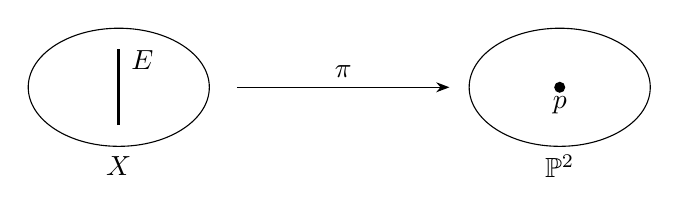
\begin{tikzpicture}[>=Stealth]
\draw (-3.4,0) ellipse (1.15 and .75);
\draw[very thick] (-3.4,-.48)--(-3.4,.48);
\node at (-3.1,.35) {\(E\)};
\node at (-3.4,-1) {\(X\)};
\draw[->] (-1.9,0)--(.8,0) node[midway,above] {\(\pi\)};
\draw (2.2,0) ellipse (1.15 and .75);
\fill (2.2,0) circle (2pt) node[below] {\(p\)};
\node at (2.2,-1) {\(\Pj^2\)};
\end{tikzpicture}
\end{center}
\[
L\cdot E=0,\qquad L^2=1,\qquad
h^0(X,L^m)=\binom{m+2}{2}.
\]
The exceptional curve has degree zero. The picture is schematic.
\end{frame}

\begin{frame}{Kawamata--Viehweg vanishing}
For a nef and big line bundle \(L\) on smooth projective \(X\),
\[
\boxed{H^q(X,K_X\otimes L)=0,\qquad q>0.}
\]
\par\bigskip
\textbf{Kawamata--Viehweg:} obtain vanishing under the weaker positivity assumptions \textquotedblleft nef and big.\textquotedblright
\par\bigskip
\par We will construct a positive singular metric with \(\cI_h=\cO_X\).
\end{frame}

\begin{frame}{Yujiro Kawamata and Eckart Viehweg}
\begin{columns}[c]
\column{.48\textwidth}
\centering
\includegraphics[width=\linewidth,height=3.6cm,keepaspectratio]{../assets/Yujiro_Kawamata.png}
\par\medskip\textbf{Yujiro Kawamata}
\par\smallskip{\small Oberwolfach, 2004}
\column{.48\textwidth}
\centering
\includegraphics[width=\linewidth,height=3.6cm,keepaspectratio]{../assets/Eckart_Viehweg.png}
\par\medskip\textbf{Eckart Viehweg}
\par\smallskip{\small Oberwolfach, 2009}
\end{columns}
\par\bigskip
\centering Independent vanishing theorems in 1982:\\ positivity can be weakened to \textbf{nef and big}.
\src{Photos: Renate Schmid / MFO, CC BY-SA 2.0 DE. Papers: Math. Ann. 261 (1982), 43--46; J. reine angew. Math. 335 (1982), 1--8.}
\end{frame}

\begin{frame}{Plan for Kawamata--Viehweg}
\begin{enumerate}
\setlength{\itemsep}{14pt}
\item Bigness writes a power of \(L\) as an ample bundle times an effective divisor bundle.
\item Nefness lets us increase that power while keeping the divisor fixed.
\item Take a large root of the metric. Its pole becomes weak enough to be integrable.
\item The multiplier ideal is trivial. Apply Nadel.
\end{enumerate}
\end{frame}

\begin{frame}{Bigness provides an ample part}
\textbf{Kodaira's lemma, in the form we need.}
For a big \(L\), there are a very ample divisor \(A\), an integer \(d>0\), and an effective divisor \(D\) such that
\[
\boxed{L^d\simeq\cO_X(A+D).}
\]
\par\bigskip
A sufficiently large power contains a fixed ample contribution.
\par\medskip
We keep \(A,D,d\) fixed from now on.
\src{Projective input: Kodaira's lemma. See Demailly, CIME notes, Proposition 6.6(f) and its proof.}
\end{frame}

\begin{frame}{Step 1: what does the effective divisor mean?}
Kodaira's lemma gives
\[
L^d\simeq\cO_X(A)\otimes\cO_X(D),\qquad D\ge0.
\]
\textbf{The ample part} \(\cO_X(A)\) has a smooth positive metric.
\par\bigskip
\textbf{The effective divisor} \(D\) is the zero set, with multiplicities, of a nonzero section of \(L^d\otimes\cO_X(-A)\).
\par\bigskip
The short dimension argument proving this lemma is in the appendix.
For now keep \(A,D,d\) fixed.
\end{frame}

\begin{frame}{Step 2: increase the power, keep the divisor}
For any integer \(N>d\),
\[
L^N=L^{N-d}\otimes L^d.
\]
Substitute the decomposition from Kodaira's lemma:
\[
L^N=\underbrace{L^{N-d}\otimes\cO_X(A)}_{M_N}\otimes\cO_X(D).
\]
The divisor \(D\) is still the same divisor. Only \(M_N\) changes.
\end{frame}

\begin{frame}{Step 2: this is where nefness enters}
We use the projective fact
\[
\boxed{\text{nef}\otimes\text{ample}\quad\text{is ample}.}
\]
Since \(L^{N-d}\) is nef and \(\cO_X(A)\) is ample,
\[
M_N=L^{N-d}\otimes\cO_X(A)
\]
is ample.
\par\medskip
Choose a smooth positive metric \(h_N\) on \(M_N\).
\src{Projective input: Demailly, CIME notes, Proposition 6.2(b).}
\end{frame}

\begin{frame}{Step 3: the metric of an effective divisor}
Locally, write the section defining \(D\) as \(s_D=f_D e_D\), where \(e_D\) is a holomorphic frame of \(\cO_X(D)\).
\par\medskip
Give this frame the squared norm
\[
\boxed{|e_D|_{h_D}^2=|f_D|^{-2}.}
\]
Then, away from \(D\),
\[
|s_D|_{h_D}^2=|f_D|^2|f_D|^{-2}=1.
\]
The metric becomes singular along the zero set of \(f_D\).
\end{frame}

\begin{frame}{Step 3: why its curvature is nonnegative}
Write the divisor metric as
\[
h_D=|f_D|^{-2}=e^{-2\log|f_D|}.
\]
Its weight is \(\varphi_D=\log|f_D|\), so
\[
i\Theta_{h_D}=2i\partial\db\log|f_D|.
\]
Poincaré--Lelong says
\[
\boxed{2i\partial\db\log|f_D|=2\pi[D]\ge0.}
\]
Here \([D]\) is the positive current of integration over the divisor, with multiplicities.
\end{frame}

\begin{frame}{Step 3: first build a metric on the power}
Recall the bundle decomposition
\[
L^N=M_N\otimes\cO_X(D).
\]
Multiply the two metrics:
\[
H_N=h_Nh_D\qquad\text{on }L^N.
\]
Their curvatures add:
\[
i\Theta_{H_N}=\underbrace{i\Theta_{h_N}}_{>0}+\underbrace{2\pi[D]}_{\ge0}.
\]
So this singular metric on \(L^N\) has strictly positive curvature.
\end{frame}

\begin{frame}{Step 3: take the root to return to the bundle}
We need a metric on \(L\), not on \(L^N\).
\par\medskip
In a frame \(e\) of \(L\), define
\[
|e|_h^2=\left(|e^{\otimes N}|_{H_N}^2\right)^{1/N}.
\]
This is the metric denoted by
\[
\boxed{h=H_N^{1/N}=(h_Nh_D)^{1/N}.}
\]
A change \(e\mapsto ge\) multiplies its squared norm by \(|g|^2\), as required for a metric on \(L\).
\end{frame}

\begin{frame}{Step 3: what happens to curvature under a root?}
If \(H_N=e^{-2\Phi_N}\) locally, then
\[
h=H_N^{1/N}=e^{-2\Phi_N/N}.
\]
Consequently
\[
i\Theta_h=\frac1N i\Theta_{H_N}
=\frac1N i\Theta_{h_N}+\frac{2\pi}{N}[D].
\]
For each fixed \(N\), the smooth first term is positive. Compactness gives
\[
\boxed{i\Theta_h\ge\varepsilon_N\omega\quad\text{for some }\varepsilon_N>0.}
\]
Nadel needs one positive constant for our chosen \(N\).
\end{frame}

\begin{frame}{Step 3: what happens to the pole under a root?}
Locally \(h_D=|f_D|^{-2}\). Thus
\[
h=(h_Nh_D)^{1/N}
=(\text{smooth positive factor})\,|f_D|^{-2/N}.
\]
\textbf{The function \(f_D\) stays fixed. The exponent \(2/N\) gets smaller.}
\par\bigskip
This is why keeping the divisor fixed mattered.
\par\medskip
We can make its singularity milder by increasing \(N\).
\end{frame}

\begin{frame}{Step 4: an integrability example in one variable}
Suppose the divisor has equation \(f_D(z)=z^m\). The singular factor is
\[
|f_D|^{-2/N}=|z|^{-2m/N}.
\]
In polar coordinates,
\[
\int_{|z|<\delta}|z|^{-2m/N}\,dx\,dy
=2\pi\int_0^\delta r^{1-2m/N}\,dr.
\]
This is finite exactly when
\[
1-2m/N>-1\quad\Longleftrightarrow\quad N>m.
\]
A sufficiently large root makes this pole integrable.
\end{frame}

\begin{frame}{Step 4: the general integrability fact}
\textbf{Local lemma.} For a nonzero holomorphic function \(f\), there is a sufficiently small \(c>0\) such that \(|f|^{-2c}\) is locally integrable.
\par\bigskip
Apply this with \(f=f_D\) and \(c=1/N\).
\par\medskip
A finite cover of the compact divisor gives one sufficiently large \(N\), valid everywhere.
\par\bigskip
Therefore \(h=(\text{smooth factor})|f_D|^{-2/N}\) has locally integrable squared frame norms.
\src{We use the local lemma here. Its Weierstrass/Hölder proof is in the appendix.}
\end{frame}

\begin{frame}{Step 4: why the multiplier ideal is trivial}
By definition, a germ \(u\) belongs to \(\cI(h)\) when
\[
|u|^2e^{-2\varphi_h}\quad\text{is locally integrable}.
\]
We just proved that \(e^{-2\varphi_h}\) itself is locally integrable.
\par\medskip
So the constant germ \(1\) belongs to \(\cI(h)\). An ideal containing \(1\) is the whole ring:
\[
\boxed{\cI(h)=\cO_X.}
\]
\end{frame}

\begin{frame}{Step 4: Nadel gives Kawamata--Viehweg}
On the original bundle \(L\), we now have
\[
i\Theta_h\ge\varepsilon_N\omega,\qquad\cI(h)=\cO_X.
\]
Nadel therefore gives
\[
H^q(X,K_X\otimes L\otimes\underbrace{\cI(h)}_{\cO_X})=0
\qquad(q>0).
\]
Hence
\[
\boxed{H^q(X,K_X\otimes L)=0\quad(q>0).}
\]
\end{frame}

\begin{frame}{An older theorem through a newer one}
\begin{center}
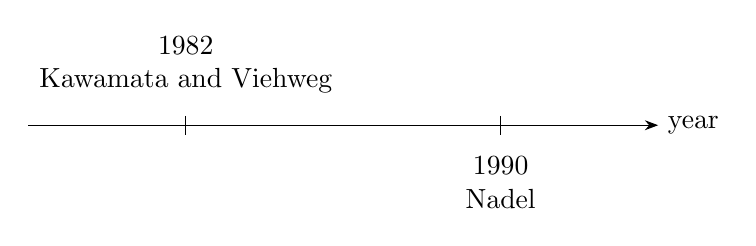
\begin{tikzpicture}[>=Stealth]
\draw[->] (-4,0)--(4,0) node[right] {year};
\draw (-2,.12)--(-2,-.12);
\node[above=8pt,align=center] at (-2,0) {1982\\Kawamata and Viehweg};
\draw (2,.12)--(2,-.12);
\node[below=8pt,align=center] at (2,0) {1990\\Nadel};
\end{tikzpicture}
\end{center}
\par\bigskip
Our proof uses the later analytic theorem to recover the earlier vanishing result.
\src{Kawamata, \emph{Math. Ann.} 261 (1982); Viehweg, \emph{J. reine angew. Math.} 335 (1982); Nadel, \emph{Annals} 132 (1990).}
\end{frame}

\begin{frame}{What the two applications have in common}
\begin{center}
\renewcommand{\arraystretch}{1.8}
\begin{tabular}{lll}
Metric & Ideal & Conclusion\\
\hline
Chosen logarithmic poles & \(\mathfrak m_x,\ \mathfrak m_x^2,\ldots\) & sections give an embedding\\
Mild divisor poles & \(\cO_X\) & ordinary vanishing
\end{tabular}
\end{center}
\par\bigskip
Positive curvature gives vanishing.
The singularities decide which ideal appears.
\end{frame}

\begin{frame}{Optional: why one cutoff bound works for all centres}
Take finitely many charts \(V_j\Subset U_j\) covering \(X\). Choose \(r_j>0\) so that \(B(z(x),2r_j)\subset U_j\) for every \(x\in V_j\).
\par\medskip
Translate one fixed cutoff \(\chi_j(z-z(x))\), equal to \(1\) on radius \(r_j\), and zero beyond \(2r_j\).
\par\medskip
On the annulus \(r_j\le|z-z(x)|\le2r_j\), all derivatives up to order two of \(a\chi_j\log|z-z(x)|\) have bounds independent of \(x\).
\par\medskip
The coordinate metrics are uniformly comparable with \(\omega\). Take the largest bound over the finite atlas and \(a=n,n+1\).
\end{frame}

\begin{frame}{Optional: what happens when the two points approach?}
The supports of \(\psi_x\) and \(\psi_y\) can overlap. We only use
\[
2i\partial\db(\psi_x+\psi_y)\ge-2C_1\omega.
\]
For each fixed \(x\ne y\), \(\psi_y\) is smooth in some neighbourhood of \(x\), so it does not change the multiplier ideal there.
\par\medskip
The same holds at \(y\). Elsewhere both weights are smooth.
\[
\cI(h)=\mathfrak m_x\cap\mathfrak m_y.
\]
We do not need disjoint supports or compactness of \(X\times X\setminus\Delta\).
\end{frame}

\begin{frame}{Why an ample part exists}
Choose a smooth very ample divisor \(A\). The sequence
\[
0\to L^m(-A)\to L^m\to L^m|_A\to0
\]
gives
\[
h^0(X,L^m(-A))\ge h^0(X,L^m)-h^0(A,L^m|_A).
\]
Bigness gives \(h^0(X,L^m)\ge c m^n\) along a subsequence, while
\(h^0(A,L^m|_A)=O(m^{n-1})\).
\par\medskip
For some \(m=d\), the kernel is nonzero. Its section has an effective zero divisor \(D\), so \(L^d(-A)=\cO_X(D)\).
\src{Additional projective inputs: Bertini and the section-growth bound on a variety of dimension \(n-1\).}
\end{frame}

\begin{frame}{Optional: why a small exponent is integrable}
By Weierstrass preparation, after choosing a suitable coordinate \(w\),
\[
f(z',w)=u(z',w)\prod_{j=1}^k(w-\alpha_j(z')),
\]
where \(u\) and \(u^{-1}\) are bounded on a smaller polydisc.
The roots need not depend holomorphically on \(z'\).
\par\medskip
Hölder's inequality bounds the \(w\)-integral of the product by
\[
\prod_{j=1}^k\left(\int |w-\alpha_j|^{-2ck}\,dA(w)\right)^{1/k}.
\]
These integrals are uniformly finite when \(ck<1\). Fubini and a finite cover finish the argument.
\end{frame}

\begin{frame}{Optional: what a positive curvature current means}
A locally integrable weight \(\varphi\) defines \(i\Theta_h=2i\partial\db\varphi\) by weak derivatives.
\par\medskip
The inequality \(i\Theta_h\ge\varepsilon\omega\) means
\[
\langle i\Theta_h-\varepsilon\omega,\eta\rangle\ge0
\]
for every smooth compactly supported strongly positive test form \(\eta\) of bidegree \((n-1,n-1)\).
\par\medskip
For smooth curvature, this is exactly the usual nonnegativity of the associated Hermitian form. For singular curvature, it remains meaningful without pointwise coefficients.
\end{frame}

\end{document}
